\documentclass{article}
\usepackage[utf8]{inputenc}

\title{CS 376 : Assignment 6 \\
Modeling and Simulation of Petri Nets}
\author{Fred Eisele }
\date{29 October 2014}

\usepackage{graphicx}
\usepackage{mathtools}

\begin{document}

\maketitle

\section{Introduction} \label{sec:intro}
A tourist agency is setting up boat sightseeing tour
where the boats are autonomous vehicles.
You have been employed by the agency to design a control
system that drives the boat along the channels
as described in the following map.


\begin{figure}[h!]
\centering
\includegraphics[scale=0.5]{boat_tour.png}
\caption{Boat Tour}
\label{fig:boat-tour}
\end{figure}

\paragraph
The channel, Figure \ref{fig:boat-tour},
has been divided up into regions.
In the Petri-nets, Figures \ref{fig:pn1}
\ref{fig:pn2} and \ref{fig:pn3}, the places
with names following the pattern $P#$
represent these regions.
The exception to this rule is the $P3A$ and $P3B$
places which represent region #3.
In that case the place represents the path
through the region with $P3A$ representing the
lower path and $P3B$ representing the upper path.
The transitions are named based on the
boundaries between the regions $T##$ where
the first digit is the start region and the
second digit the destination.
A token in any of these places represents a boat.
Tokens in other places represent permision (not boats).


\section{Single Boat Indeterminate Path} \label{sec:1-indet}

Model the problem of a single boat with a Petri net
and describe in detail what each place and transition represents

\begin{figure}[h!]
\centering
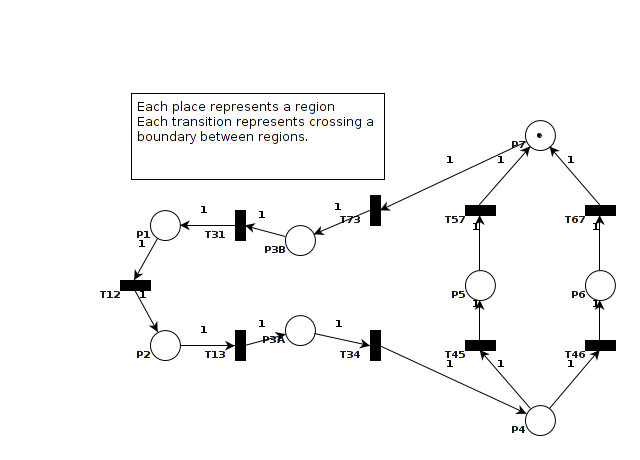
\includegraphics[scale=0.5]{hw6_petri_net_1.png}
\caption{Single Boat with Indeterminate Path}
\label{fig:pn1}
\end{figure}

\paragraph
The formal Petri net is a 5-tuple,

\begin{equation}
PN = (P, T, F, W, M_0)
\end{equation}

\ldots alternatively \ldots

\begin{align}
N &= (P, T, F, W) \\
PN &= (N, M_0)
\end{align}

Where for this model \ldots

The set of places representing the regions in the canal.
\begin{align}
P_{canal} & = \{ P1, P2, P3A, P3B, P4, P5, P6, P7 \} \\
P & = P_{canal}
\end{align}

The set of transitions representing the region boundaries.
\begin{align}
T_{canal} & = \{ T12, T23, T34, T45, T46, T57, T67, T73, T31 \} \\
T & = T_{canal}
\end{align}

The set of arcs representing the direction of movement across the region boundaries. As all weights are $1$ it is not explicitly written in
the following arc tuples rather it is implicit.
\begin{align}
PT_{canal} & = \{ (P1, T12), (P2, T23), (P3A, T34), (P4, T45),
       (P4, T46), (P5, T57), (P6, T67), (P7, T73), (P3B, T31) \} \\
TP_{canal} & = \{ (T12, P2), (T23, P3A), (T34, P4), (T45, P5),
       (T46, P6), (T57, P7), (T67, P7), (T73, P3B), (T31, P1) \} \\
F & = PT_{canal} \cup TP_{canal}
\end{align}

This completes the structural model for this problem there
are a number of valid initial markings.  An acceptable marking
would be a single token in any of the $P_{canal}$ places.

\paragraph
This produces an indeterminate path as when
there is a token in $P4$ both $T45$ and $T46$ are enabled.

\section{Single Boat Determinate Path} \label{sec:1-det}

The tourist agency wants the
boat to pass alternatively through region 5 and 6.
The Petri net in Section \ref{sec:1-indet} is
modified so that this constraint is satisfied.

\begin{figure}[h!]
\centering
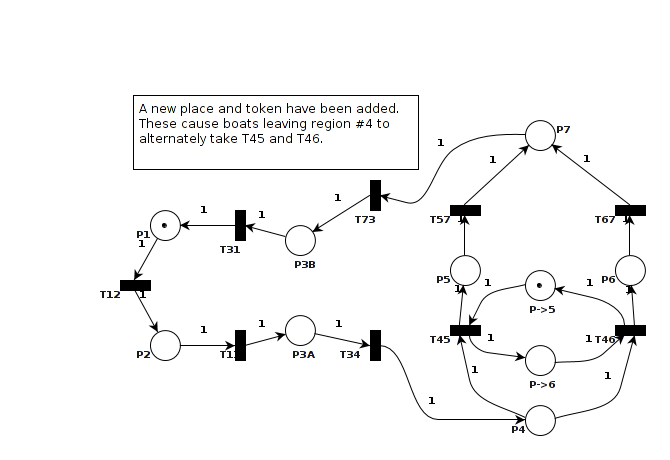
\includegraphics[scale=0.5]{hw6_petri_net_2.png}
\caption{Single Boat with Determinate Path}
\label{fig:pn2}
\end{figure}

This is done by introducing a pair of places,
$P->5$, $P->6$ and a token.
The token acts as a permit for the boat
to enter either $P5$ or $P6$
depending on whether it is in place $P->5$ or $P->6$.


The set of places representing the next alternative are added.
\begin{align}
P_{alternate} & = \{ P->5, P->6 \} \\
P & = P_{canal} \cup P_{alternate}
\end{align}

No new transitions are required.
However new arcs are required (again all weights are $1$).
\begin{align}
PT_{alternate} & = \{ (P5->5, T45), (P->6, T46) \} \\
TP_{alternate} & = \{ (T45, P->6), (T46, P->5) \} \\
F & = PT_{canal} \cup TP_{canal} \cup PT_{alternate} \cup TP_{alternate}
\end{align}

The initial marking now needs a new token in either
$P->5$ or $P->6$ but not both.


\section{Two Boats Place Exclusion} \label{sec:2-excl}

There are two boats.
This Petri-net models a system like that of
Section \ref{sec:1-det} but it additionally
only allows one boat to access region 3 at a time.

\begin{figure}[h!]
\centering
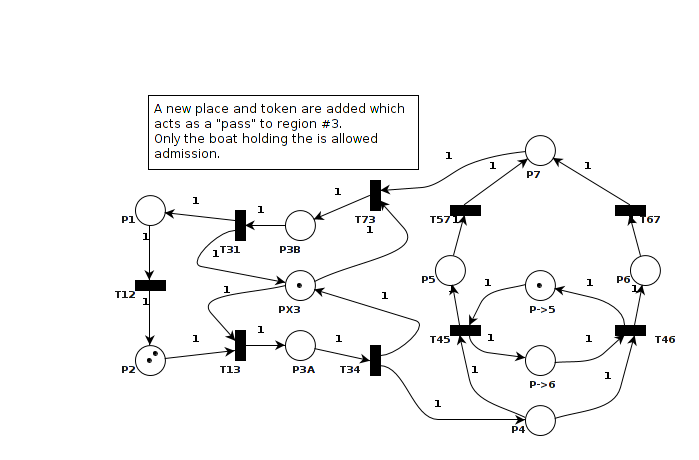
\includegraphics[scale=0.5]{hw6_petri_net_3.png}
\caption{Two Boat with Exclusion Zone and Determinate Path}
\label{fig:pn3}
\end{figure}

\paragraph
This is done by introducing a place,
$PX3$ and a token.
The token acts as a permit for the boat
to enter $P3A$ or $P3B$.
Recall that these two places represent one region.
For this reason the two places compete for the net token.


The place holding the exclusion token is added.
\begin{align}
P_{exclusion} & = \{ PX3 \} \\
P & = P_{canal} \cup P_{alternate} \cup P_{exclusion}
\end{align}

No new transitions are required.
However new arcs are required (again all weights are $1$).
\begin{align}
PT_{exclusion} & = \{ (PX3, T73), (PX3, T23) \} \\
TP_{exclusion} & = \{ (T31, PX3), (T34, PX3) \} \\
F & = PT_{canal} \cup TP_{canal} \cup PT_{alternate} \cup TP_{alternate}
    \cup PT_{exclusion} \cup TP_{exclusion}
\end{align}

The initial marking now needs a new token in
$PX3$ unless there is a token in either $P3A$ or $P3B$.
In addition the $P_{canal}$ places may contain more than
one token (the problem calls for exactly $2$).
However, there may be at most one token in $P3A \cup P3B$.


\end{document}
